\section{The Parallel Algorithm}
\label{sec:parallel-algorithm}

\subsection{MPI Preliminaries}

We define and assume the following with regard to using the Message Passing Interface (MPI) \citep{mpi40}. A {\em rank} is a compute unit with a separate, unique memory space. Each rank in the execution of a program runs a separate version of the program. {\em Communication} refers to how data is transferred between ranks via {\em messages} (or packets of data). Communication is done with actions such as sending, receiving, or broadcasting messages. A {\em communicator} is a union of ranks in which each rank has a unique index $R_i = 0, ..., N_{R}-1$, where $N_R$ is the number of ranks in a communicator. In every MPI program, there is a global communicator called {\tt MPI\_COMM\_WORLD} that contains all ranks that are executing the program.

\subsection{Quadtree Data Structures}
\label{sub:quadtree-data-structures}

\begin{figure}
    \centering
    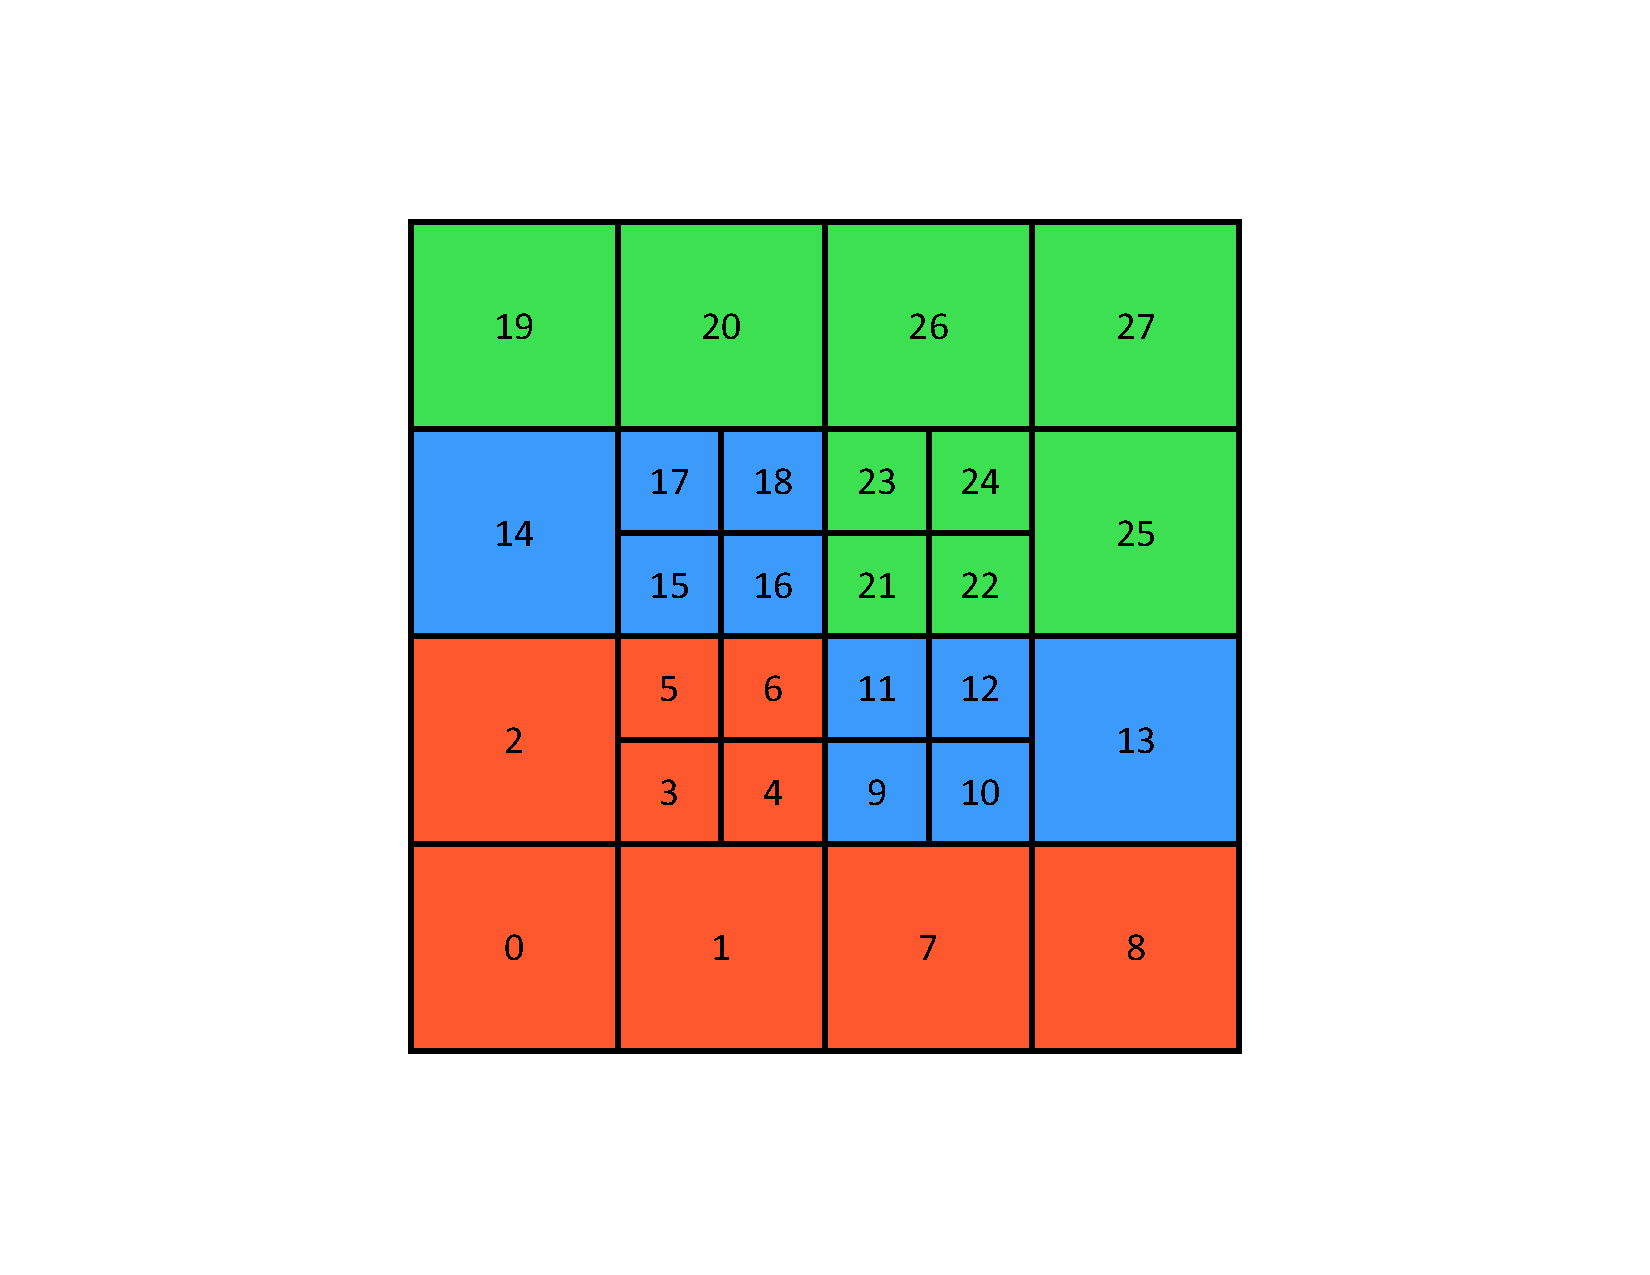
\includegraphics[width=\textwidth, clip=true, trim={0 100 0 100}]{figures/parallel_adaptive_mesh_indexing.pdf}
    \caption{An example of an adaptive, quadtree mesh that is refined around the center of the domain. The colors denote different ranks and the numbers indicate the leaf-index of the quadrant.}
    \label{fig:adaptive_mesh}
\end{figure}

\begin{figure}
    \centering
    \begin{subfigure}[t]{1\textwidth}
        \centering
        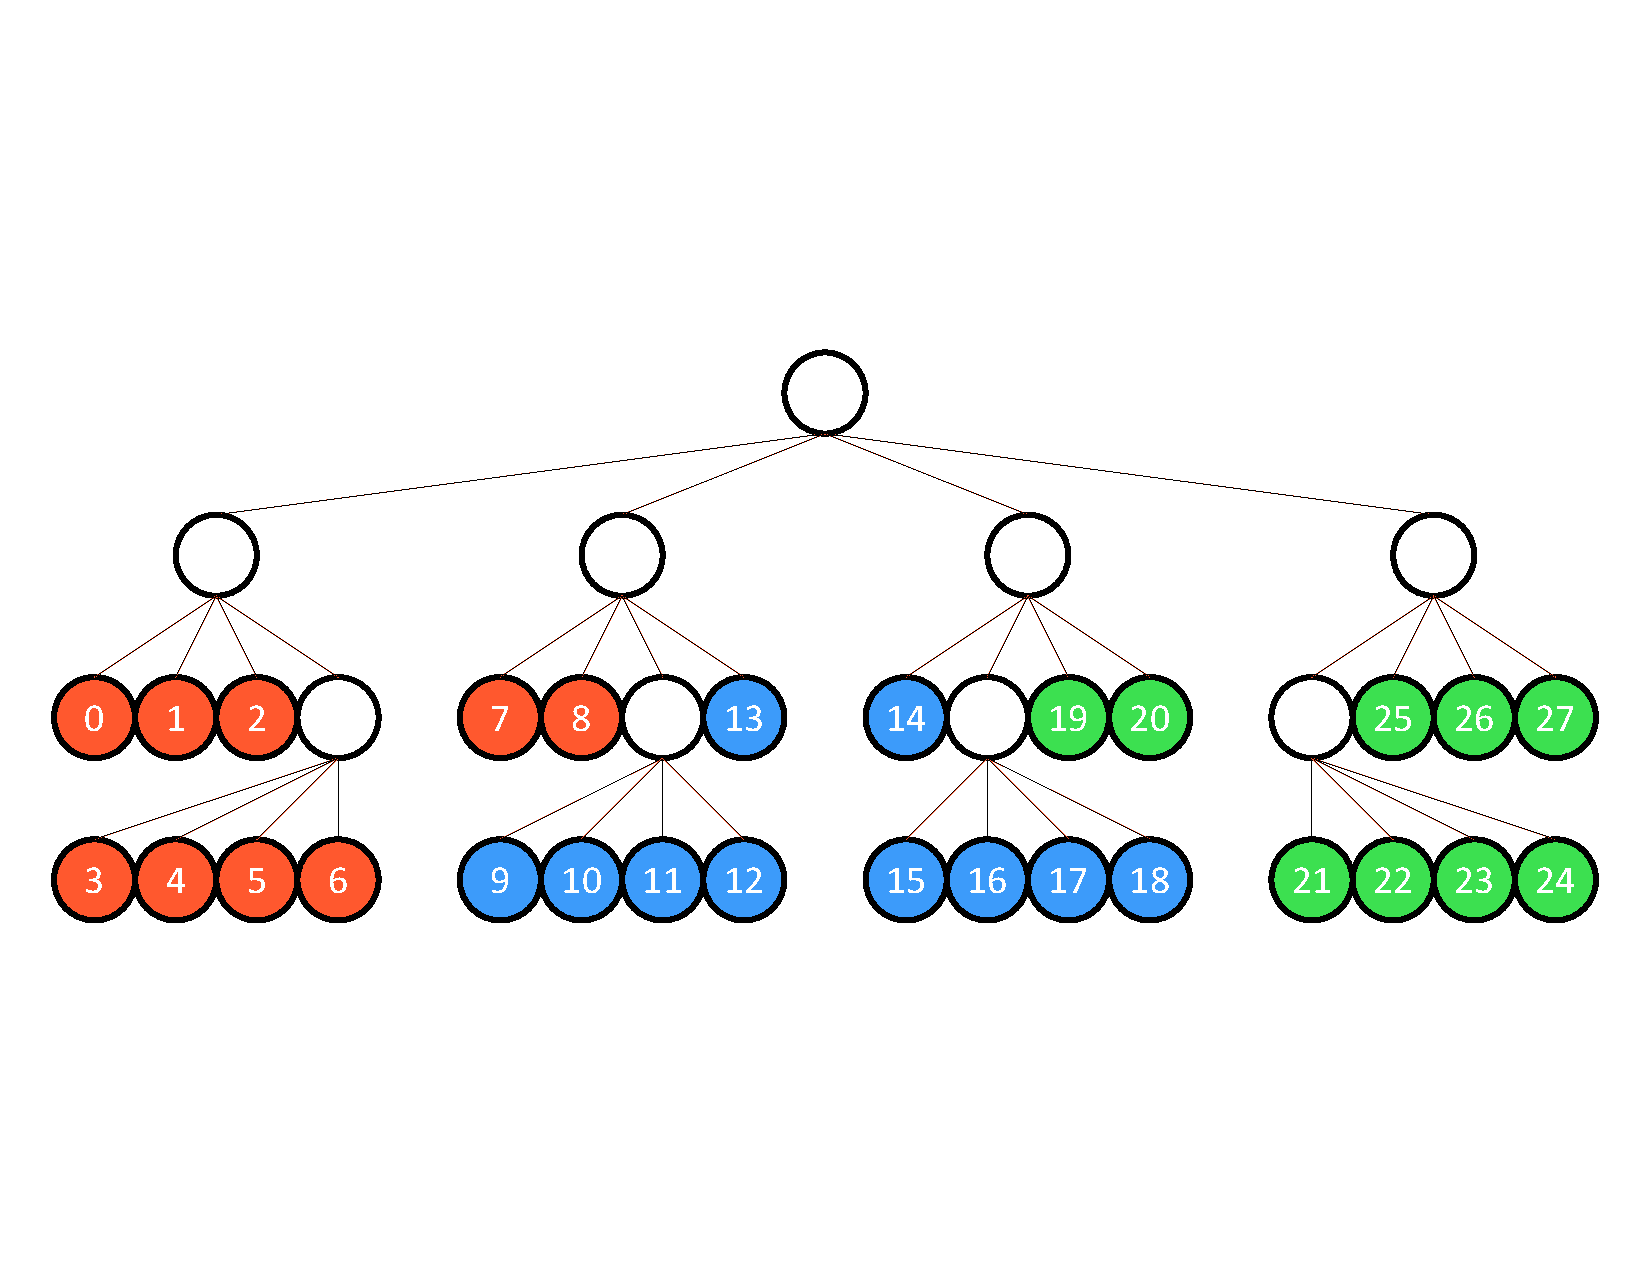
\includegraphics[width=\textwidth, clip=true, trim={0 150 0 150}]{figures/parallel_leaf_indexed_tree.pdf}
        \caption{Leaf-indexed quadtree in parallel}
        \label{subfig:leaf-indexed-quadtree}
    \end{subfigure}
    \begin{subfigure}[t]{1\textwidth}
        \centering
        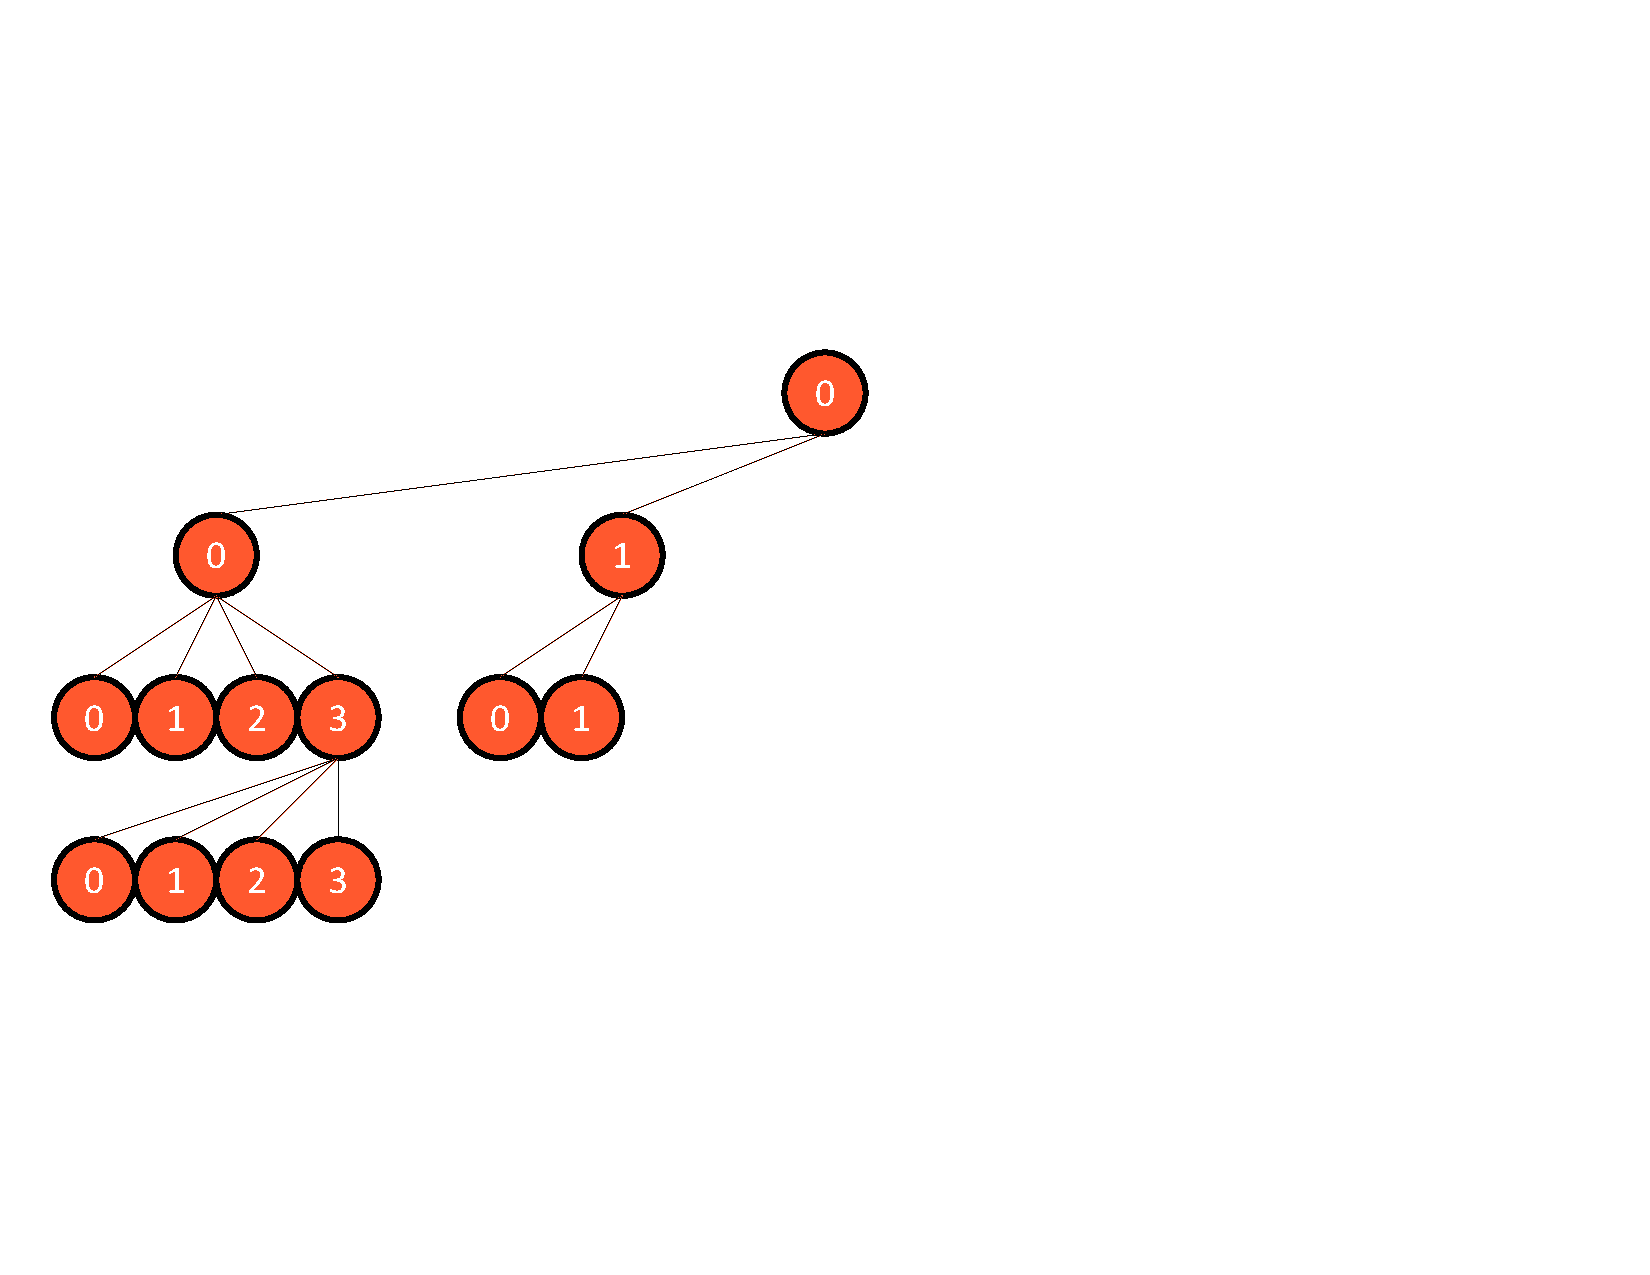
\includegraphics[width=0.32\textwidth, clip=true, trim={20 160 370 160}]{figures/parallel_path_indexed_tree0.pdf}
        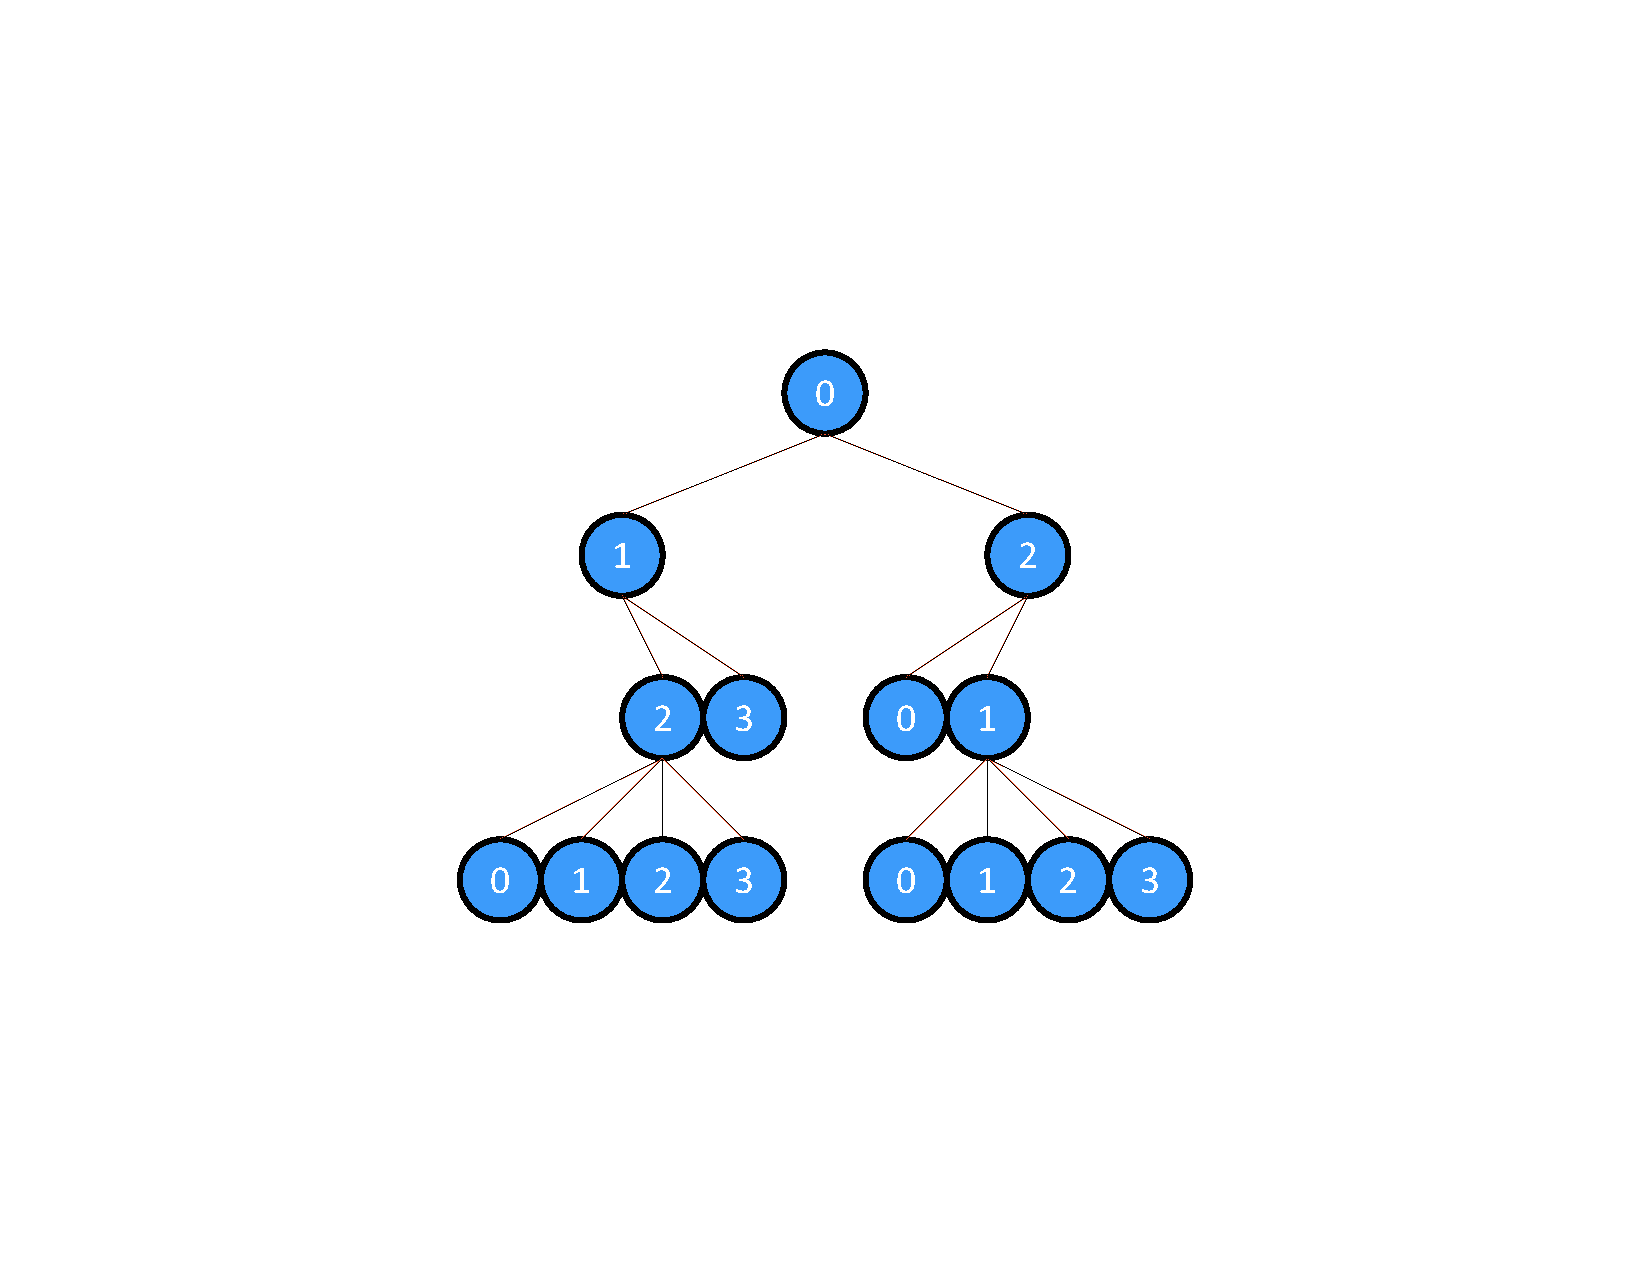
\includegraphics[width=0.32\textwidth, clip=true, trim={195 160 195 160}]{figures/parallel_path_indexed_tree1.pdf}
        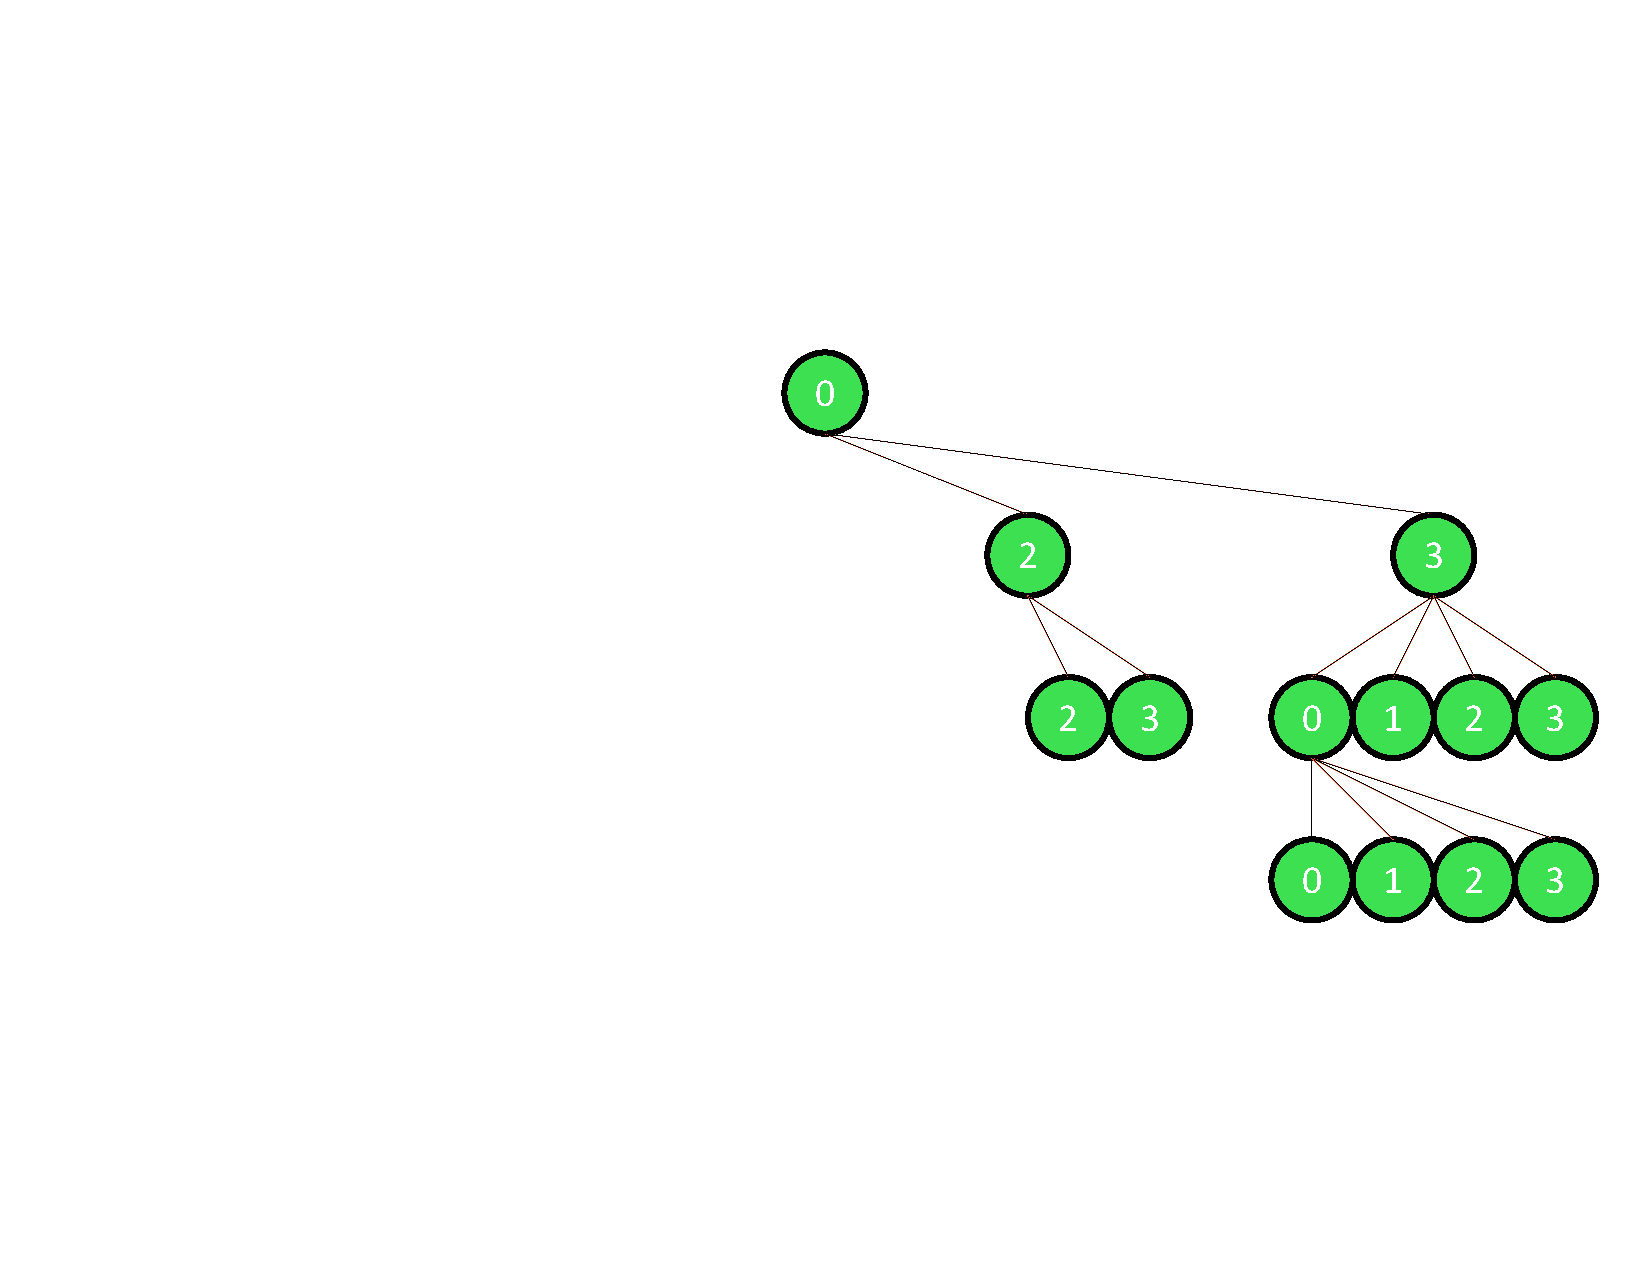
\includegraphics[width=0.32\textwidth, clip=true, trim={370 160 20 160}]{figures/parallel_path_indexed_tree2.pdf}
        \caption{Path-indexed quadtree in parallel}
    \end{subfigure}
    \caption{Leaf-indexed vs. path-indexed quadtrees. Both trees represent the mesh found in \reffig{fig:adaptive_mesh}. The colors denote which rank owns each node. In (a), only the leaves of a quadtree are indexed and stored. In (b), all nodes of the quadtree are indexed and stored according to their unique path.}
    \label{fig:quadtree_indexing}
\end{figure}

The \pforest library provides a leaf-indexed quadtree data structure and functions to construct, store, and iterate over leaf-level nodes (also called quadrants). The \pforest quadtree only stores leaf-level quadrants. These are maintained as a disjoint union over the ranks, with minimal redundant metadata stored on each rank to encode the parallel boundaries within the tree. The quadrants are stored in a rank-local array, split between the rank-relevant trees if there is more than one tree, and ordered according to a space-filling curve. Partitioning in \pforest results in an equally-divided quadtree where each rank has roughly the same number of quadrants, subject to the integer division of the number of leaf-nodes $N_{L}$ into $N_{R}$.

As outlined in \refsec{sec:problem-statement}, the \gls{qahps} method requires storage for all nodes in a quadtree, which is done through a path-indexed quadtree. This is the same in parallel. The partitioning of a path-indexed quadtree follows the partitioning of a leaf-indexed quadtree. \reffig{fig:quadtree_indexing} depicts the leaf-indexed and path-indexed quadtrees; the colors indicate which quadrants or nodes are rank-local.

The path-indexed quadtree is created by traversing the leaf-indexed quadtree in parallel. This is done with the \codename{p4est\_search\_all} function, which performs a depth-first traversal of the quadtree and calls a user provided callback function for each quadrant. The callback function provided to \codename{p4est\_search\_all} is found in \refalg{alg:p4est_search_all_callback}. The main idea of \refalg{alg:p4est_search_all_callback} is to allocate space in the path-indexed quadtree map if the provided quadrant is rank-local, and if not, set that space in the map to \codename{nullptr}. The node is created either from the root data (provided from the user) or the parent data. In practice, a factory design pattern is used to generate the nodes; the user implements a node factory object. The function \codename{p4est\_quadrant\_ancestor\_id} is a utility used to compute the index of a quadrant's ancestor.

\begin{algorithm}
    \caption{\codename{SearchAllCallback} Function (passed to \codename{p4est\_search\_all})}
    \begin{algorithmic}[0]
        \Require $\mathcal{Q}_{L}$, $\mathcal{Q}_{P}$, $\Omega_i$, $R_{\text{first}}$, $R_{\text{last}}$
        \State Get \codename{map} from $\mathcal{Q}_{P}$
        \State Compute \codename{path} from \codename{p4est\_quadrant\_ancestor\_id}($\Omega_i$)
        \State Let \codename{owned} = $R_{\text{first}} < r < R_{\text{last}}$
        \If {\codename{owned}}
            \If {$\Omega_i$ is the root quadrant}
                \State Create \codename{node\_ptr} from root data: \codename{node\_ptr} $\rightarrow \Omega^{\tau}$
            \Else
                \State Create \codename{node\_ptr} from parent data: \codename{node\_ptr} $\rightarrow \Omega^{\tau}$
            \EndIf
            \State Let \codename{map[path] = node\_ptr}
        \Else
            \State Let \codename{map[path] = nullptr}
        \EndIf
    \end{algorithmic}
    \label{alg:p4est_search_all_callback}
\end{algorithm}

Any node in a path-indexed quadtree is rank-local to a range of ranks denoted by \rfirst to \rlast. A leaf node is always local to a single rank, or \rfirst $=$ \rlast. The parents and ancestors of leaf nodes can exist across multiple ranks depending on the range of ranks of a node's descendants. The range of ranks is provided from \pforest upon initialization of the path-indexed quadtree and associated nodes.

The range of ranks allows for creation of a {\em node communicator}. A node communicator is a subset of the global communicator that includes only the range of ranks a particular node lives on. When communication is necessary (as in the 4-to-1 merge or the 1-to-4 split algorithms), a node may communicate its data to all ranks that store a version of that node in the quadtree. Creation of the node communicator is a collective routine on all ranks that are part of the super communicator. The node communicators are created and stored on each node during the initialization of the path-indexed quadtree to avoid global communication when performing the factorization or solves.

The merging and splitting algorithms detailed in \refsec{sub:stages-of-the-quadtree-adaptive-hps-method} require references to the data stored on the parent node and the children nodes associated with the merge or split. When children nodes are not rank-local, communication is necessary to share the data across ranks. Ranks within a node communicator broadcast their associated data to other involved ranks to ensure that each rank has a local copy of all children and parent nodes.

% For example, from \reffig{fig:quadtree_indexing}(b), when merging children nodes ``0210'', ``0211'', ``0212'', and ``0213'' into parent node ``021'', the yellow rank must broadcast nodes ``0210'', ``0211'', and ``0212'' to the green rank, and the green rank must broadcast node ``0213'' to the yellow rank. Both yellow and green ranks would already have storage for the parent node ``021''.

\subsection{Parallel Merge and Split Traversals}

The merge and split traversals are outlined for the serial case in \refsec{sub:quadtrees-and-adaptive-meshes}. In parallel, a family of nodes may not have all siblings on the same rank. Thus communication is necessary during merge and split traversals to ensure that node data is rank-local.

The parallel version of \refalg{alg:merge-split-callback-serial} is detailed in \refalg{alg:merge-split-callback-parallel}. This is the function that is passed to \codename{p4est\_search\_reorder} either for the pre-quadrant callback (splitting algorithms) or for the post-quadrant callback (merging algorithms). The primary logic of \refalg{alg:merge-split-callback-parallel} checks if the node is a leaf or not to call either \codename{LeafCallback} or \codename{FamilyCallback} and if the node is local to the rank executing this code. In order to call \codename{MPI\_Bcast}, the root rank must be known. This is the rank that sends the data in the broadcast; all other nodes receive the data and store it in a rank-local buffer. A call to \codename{MPI\_Allreduce} for each children node communicates which rank is the root rank for that node. The call to \codename{MPI\_Bcast} provides the buffer for ranks to send and receive node data and only communicates within the node communicator.

\begin{algorithm}[t]
    \caption{\codename{MergeSplitCallback} Function (passed to \codename{p4est\_search\_reorder})}
    \begin{algorithmic}[0]
        \Require $\mathcal{Q}_{L}$, $\mathcal{Q}_{P}$, $\Omega_i$, $R_{\text{first}}$, $R_{\text{last}}$, \texttt{LeafCallback}(\texttt{leaf\_node}) \& \texttt{FamilyCallback}(\texttt{parent\_node, children\_nodes})
        \State Get \codename{map} from $\mathcal{Q}_{P}$
        \State Compute \codename{path} from \codename{p4est\_quadrant\_ancestor\_id}($\Omega_i$)
        \State Let \codename{node\_ptr} = \codename{map[path]}: \codename{node\_ptr} $\rightarrow \Omega^{\tau}$
        \State Let \codename{owned} = $R_{\text{first}} < r < R_{\text{last}}$
        \State Let \codename{children\_ptrs} = $\{\}$
        \If{$i$ $\ge$ 0 $\And$ \codename{node\_ptr} $\ne$ \codename{nullptr} $\And$ \codename{owned}}
            \State Call \codename{LeafCallback(node\_ptr)}
        \Else
            \If{$R_{\text{first}} = R_{\text{last}}$}
                \For{$i = 0, ..., 3$}
                    \State Let \codename{children\_ptrs[i] = map[path + string(i)]}
                \EndFor
            \ElseIf{\codename{owned}}
                \For{$i = 0, ..., 3$}
                    \State Let \codename{child\_ptr = map[path + string(i)]}
                    \State Communicate \codename{child\_ptr} to all ranks in \codename{node\_comm}
                    \State Let \codename{children\_ptrs[i] = child\_ptr}
                \EndFor
            \EndIf
            \If{\codename{owned}}
                \State Call \codename{FamilyCallback(node\_ptr, children\_ptrs)}
            \EndIf
        \EndIf
    \end{algorithmic}
    \label{alg:merge-split-callback-parallel}
\end{algorithm}